%-------------------------------------------------------------------------------
% File: simulator.tex
%       Epidemic Broadcast project documentation.
%
% Author: Marco Pinna, Rambod Rahmani, Yuri Mazzuoli
%         Created on 05/12/2020
%-------------------------------------------------------------------------------
\chapter{Simulator}\label{simulator}
In order to obtain experimental results for the presented scenarios, a simulator
was built using OMNeT++. This will allow us to reproduce the different scenarios
with different values for the identified parameters.\\
\section{Omnet++ and INET framework}
OMNeT++ is an extensible, modular, component-based C++ simulation library and
framework, primarily for building network simulators\footnote{https://omnetpp.org/}.\\
The INET Framework is an open-source model library for the OMNeT++ simulation
environment. It provides protocols, agents and other predefined models for
researchers and students working with communication networks. INET is especially
useful when designing and validating new protocols, or exploring new or exotic
scenarios\footnote{https://omnetpp.org/download-items/INET.html}.\\
OMNeT++ is a library and a framework, and can be used with the dedicated IDE.
Not only it allows for development of the simulator itself, but also to export
simulation results and to inspect simulation behaviour with a graphical user
interface. Exploiting C++ compiler optimizations, it can achieve the lowest
simulation duration possible. Networks are composed by modules; there are two
types of modules: simple module and compound module (which can contain other
modules itself). INET is an extension of OMNeT++, dedicated to recreating 
network simulation environments, with the capability of reproducing the activity
of a wireless communication system across multiple nodes. It contains ready to
use definitions and implementations of network related modules.\\
\\
The choice was made to use the INET framework in order to avoid spending too
much time on the coding side and therefore be able to focus more on other
aspects such as the problem modeling and analysis.
\section{Network architecture}
The network based architecture is composed by an Array of Host modules, an
Integrated visualizer (visualizer) and a UnitDiskRadioMedium (radioMedium);
\begin{figure}[H]
    \begin{center}
        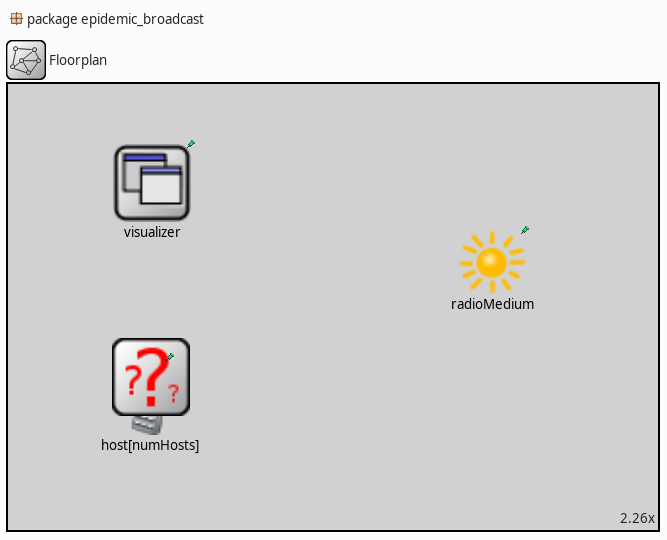
\includegraphics[scale=0.35]{img/floorplan.png}
        \caption{Floorplan.ned}
        \label{fig:single_queue}
    \end{center}
    \vspace*{-0.8cm}
\end{figure}
\begin{itemize}
    \item \textbf{UnitDiskRadioMedium} is a compound module provided by INET.
    This radio medium model provides a very simple but fast and predictable
    physical layer behavior. It must be used in conjunction with the
    \texttt{UnitDiskRadio} model. It can simulate the behaviour of the wireless
    communication channel with various levels of abstraction.
    \item \textbf{Integrated visualizer} is a compound module provided by INET.
    It's resposible for the visual representation of modules properties and
    events in the graphic user interface.
    \item \textbf{Host} is the compound module developer for representing a node
    in our network environment.
\end{itemize}
The \texttt{Host} module extends the NodeBase module defined by INET. This
module contains the most basic infrastructure for network nodes that is not
strictly communication protocol related. The following diagram shows usage
relationships between types:
\begin{figure}[H]
    \begin{center}
        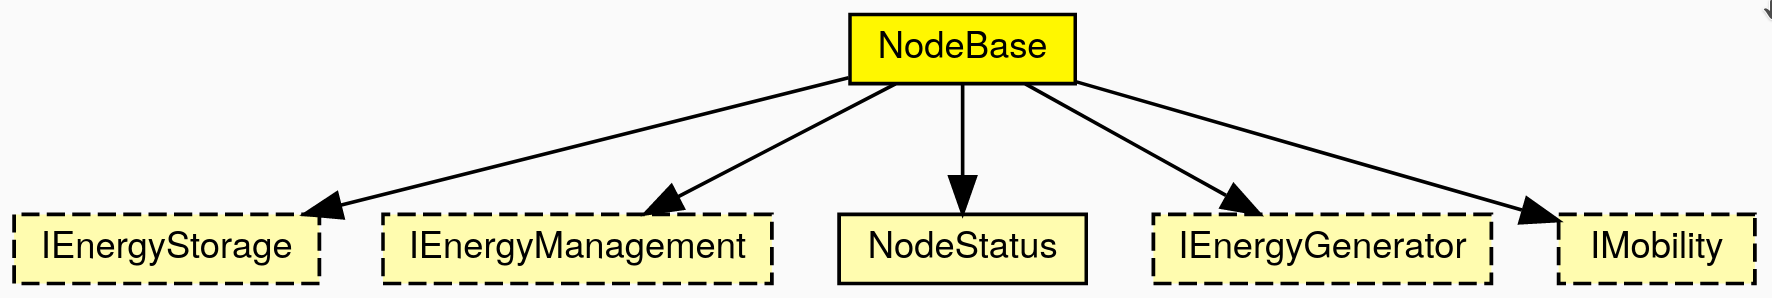
\includegraphics[scale=0.26]{img/nodebase.png}
        \caption{NodeBase Diagram.}
        \label{fig:single_queue}
    \end{center}
    \vspace*{-0.8cm}
\end{figure}
\begin{figure}[H]
    \begin{center}
        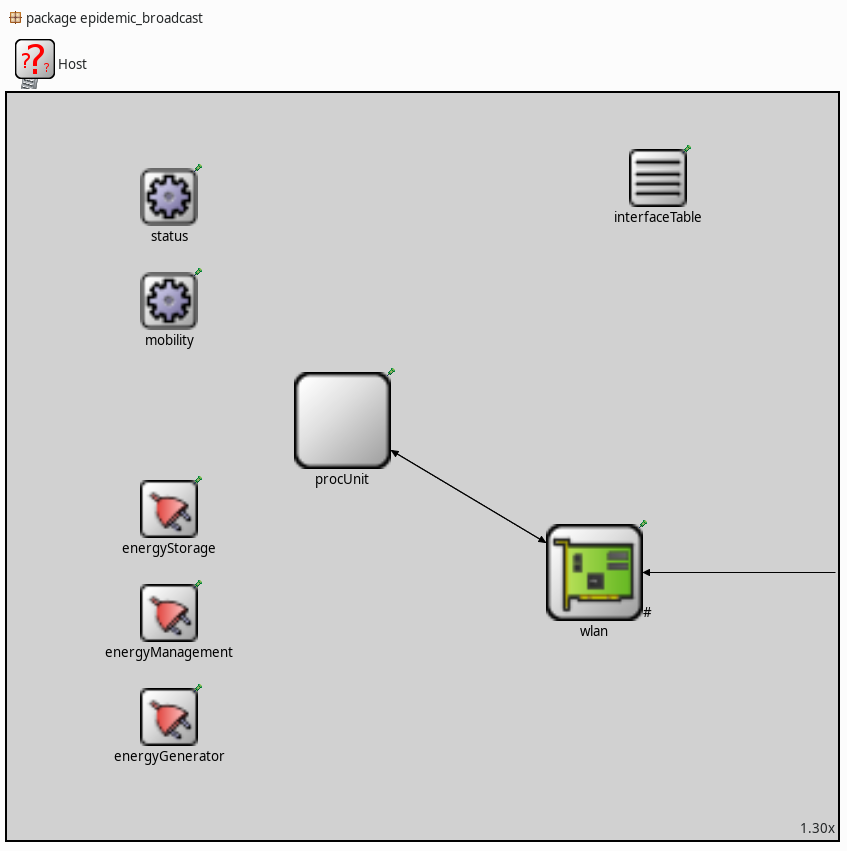
\includegraphics[scale=0.35]{img/host.png}
        \caption{host.ned}
        \label{fig:single_queue}
    \end{center}
    \vspace*{-0.8cm}
\end{figure}
\begin{itemize}
    \item the \texttt{mobility} module privided by INET manages the position of
    the parent module \texttt{Host}; it allows various types of movements, but
    we are going to be using it only for the initial random placement of the
    nodes, then all nodes will be stationary.
    \item the \texttt{interfaceTable} module is provided by INET and is required
    for correct operation of the radioMedium module.
    \item the \texttt{wlan} module is the wireless interface that allows nodes
    to communicate with each others. It's an \texttt{AckingWirelessInterface}
    compound module, which is the simplest wireless interface provided by INET.
    \item the \texttt{status} module is provided by INET as well and is required
    to shutdown and restart network interfaces.
    \item the \texttt{procUnit} module is the custom made processing unit, that
    implements the node behaviour when a message arrives. It's connected to the
    \texttt{wlan} module in order to be able to receive and send messages.
    \item \texttt{energyStorage}, \texttt{energyManagement} and
    \texttt{energyGenerator} are modules inherited from \texttt{NodeBase} but
    they are not instantiated as we don't need to model energy related
    behaviours.
\end{itemize}
The \texttt{wlan} module is in charge of checking each and every message for
collisions, and drop broken packets instead of forwarding them to the processing
unit. The processing unit \texttt{ProcUnit} implements the behaviours of the
nodes; it handles the broadcast message when received, and then its
retransmission when the random variable extraction results in a success. Finally
it shuts down the network interface, preventing it from receiving any messages
or provoking collisions. The network interface is turned off also for the entire
duration of the RV extractions.
\section{Parameters and Statistics}
During the simulation, signals are used to collect the statistics. They are all
collected by the \texttt{Flooplan} module:
\begin{itemize}
    \item The \texttt{wlan} module emits a signal every time a collision is
    detected; this signal is collected by the
    \texttt{packetDropIncorrectlyReceived} statistic of the same module; we are
    interested in the total number of collisions detected by each node.
    \item The \texttt{ProcUnit} module emits $2$ signals when initialized,
    \texttt{hostX} and \texttt{hostY}, collected, respectively, by the
    \texttt{hostXstat} and \texttt{hostYstat} statistics; those are the
    coordinates of the parent node in the floorplan.
    \item The \texttt{ProcUnit} module emits the \texttt{timeCoverage} singal as
    well, collected in the \texttt{timeCoverageStat} statistic; this is a
    vector containing, for each node that received the broadcast message, the
    number of the time slot when the broadcast message was actually received; at
    the end of the simulation, it's size represents the number of covered nodes.
    \item The \texttt{ProcUnit} module emits the \texttt{coverage} singal too;, collected by the Flooplan module in the \texttt{coverageStat} statistic; 
        this sum also represent the number of nodes covered at the end of the simulaton.
\end{itemize}
Most significative parameters set up in the initialization file (floorplan.ini) are reported belaw:
%snapshot del file ini con gli sweep per p ed r, e altri parametri più significativi 
\section{Design Choises and Optimizations}
The utilization of INET framework for simulator developement allow us to exploit a pre-builted model for wireless communications;
for example, collision detection and statistic collection about it is already implemented in INET modules. During the developement
we choise for every aspect the optimal level of abstraction for owr purpose, but it's possible to model other aspects just 
changing typse to the INET modules, or adding new ones. We voluntarily omitted phenomena like pathloss and node movement, and we 
restrict owr considerations to a discrete time scenario, but it will be very easy to model this complex things just changing
few modules types and attributes. \\
INET modules have also pre-builted optimizaton structures, that become indispensable when the number of modules become large; in order
to make the simulator ready for high complex scenarios we used an the \textbf{neighborCache} structure offered by the radioMedium module.
This module is in charge of store the proximity information of every nodes, in order to speed up messages delivery. Setting the type of this
module to \texttt{GridNeighborCache} it's possible to reduce the time needed for a simulaton with more than 2000 devices, by a factor of 
10; we also found that this particulare type of cache (with the right cellSize) is the best trade-off beetween speed and memory occupancy,
for this type of workload\footnote{https://doc.omnetpp.org/inet/api-current/neddoc/inet.physicallayer.contract.packetlevel.INeighborCache.html}.  
